\section{Visualisation}
An interactive application was built to visualise the results. The application operates like a dashboard, allowing the user to make real-time adjustments to the circuit parameters. The circuit's behavior is then simulated accordingly, and the results are dynamically plotted on the graphs with respect to time. This interactive approach enables the user to gain insights into the circuit's performance by visualizing node voltages ($e_2$, $e_3$), currents ($i_z$, $i_l$, $i_d$, $i_c$, $i_s$), and the power dissipation in resistor $R_s$.

\begin{figure}[H]
     \centering
     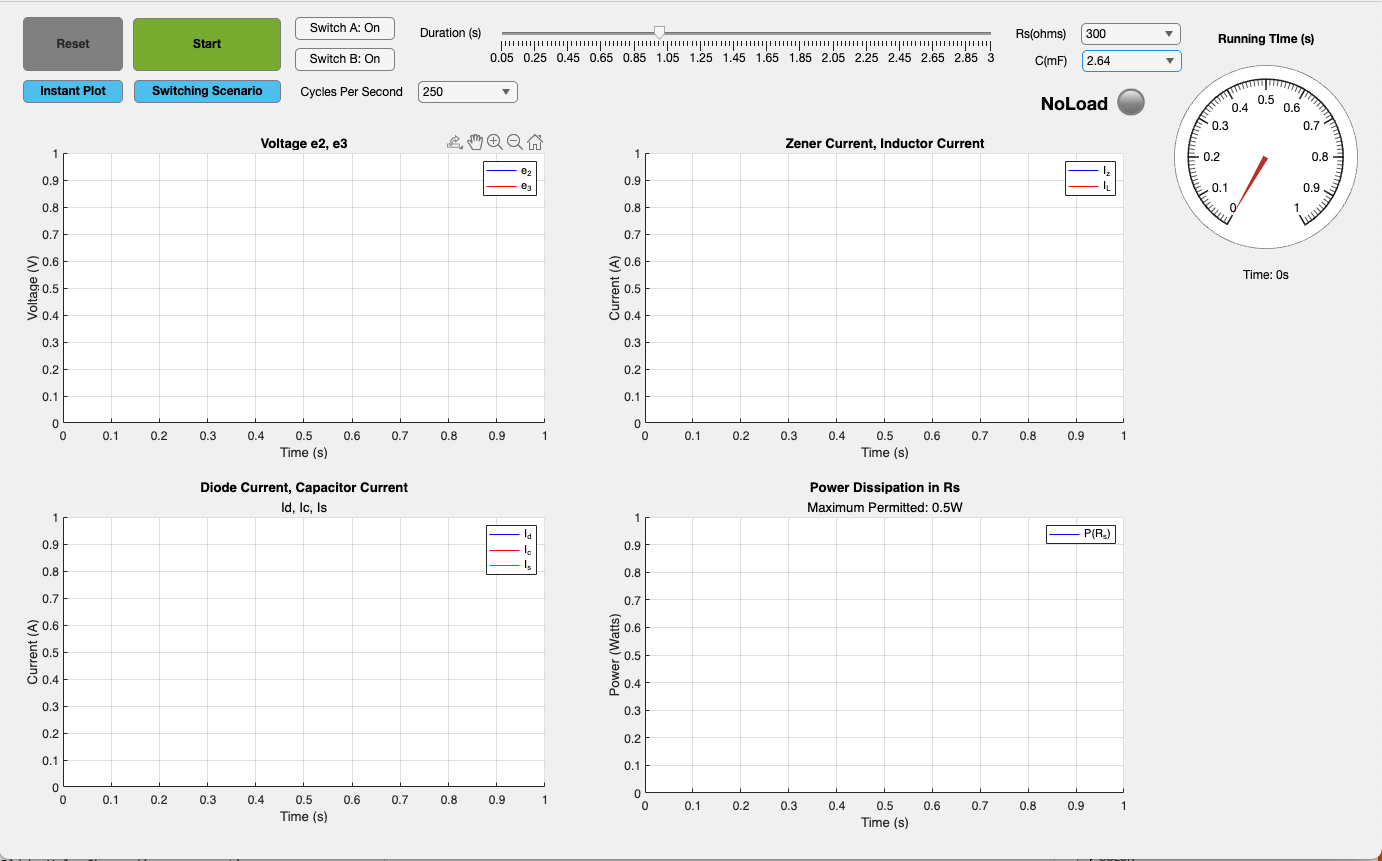
\includegraphics[width=15cm]{graphics/visualisation/inactive_ui}
     \caption{User interface of the visualisation while it is inactive}
\end{figure}
The operation mode of the simulation is determined by the switching of the primary and secondary switches in the multi-mode load, as depicted in Figure \ref{fig:multimode_load}. The user can toggle the switch buttons to change the switching operation dynamically, even while the simulation is running. This enables the user to explore different scenarios and observe the corresponding effects on the circuit's behavior.

\leavevmode\newline
Furthermore, the application supports the adjustment of several parameters. The user can modify the capacitance ($C$) and resistance ($R_s$) values within their nominal, maximum, and minimum ranges, as specified in Table \ref{tab:component_values}. Additionally, the sampling rate ($c$), which determines the time step ($h$) used in the simulation's numerical method (RK4), can be adjusted. Lastly, the user can specify the duration of the simulation, allowing them to observe the circuit's behavior over a desired period.

\leavevmode\newline
To provide real-time feedback to the user, a status indicator is employed to indicate the current mode of operation based on the switch toggles. Additionally, a time gauge is included to keep track of the running simulation time, allowing the user to monitor the progress of the simulation. Control buttons are provided to start, pause, resume, and reset the simulation. These buttons offer convenient control over the simulation's execution and allow the user to pause and resume at any point or start a fresh simulation whenever desired.

\subsection{Implementation}
This MATLAB visualisation application uses AppDesigner to build an interactive user interface for exploring power supply characteristics in different operating modes. It uses a \texttt{ComponentContainer} class which provides a high-level abstraction for the graphical interface, encapsulating the visual components as properties and methods of the class.
\\

Three key functions have been included as code extracts to help illustrate the inner workings and implementation details of the visualisation application. These code snippets highlight specific functions that play crucial roles in enabling the interactive features and simulation capabilities of the application.

\subsubsection{postSetupFcn}
This function, called immediately after the initialization of the application, performs essential setup tasks to configure the initial state of the simulation and prepare the necessary elements for plotting. It establishes the initial conditions, defines the time range, and creates animated lines for each plot.

\begin{lstlisting}[caption=MATLAB code for the function called imeddiately after the UI is initialised]
function postSetupFcn(comp)
% Set initial state
comp.Running = false; 
comp.Paused = false;
comp.t = 0:comp.TimeStep:comp.Duration;
comp.k = 1;
comp.v = @(t) 230 * sqrt(2) * sin(100*pi*t);
comp.ic = [0,0,0];

% Create animated lines for each plot
comp.l_e2 = animatedline(comp.VoltagePlot,Color='b');
comp.l_e3 = animatedline(comp.VoltagePlot,Color='r');
comp.l_iZ = animatedline(comp.VoltagePlot,Color='m');
comp.l_iD = animatedline(comp.DiodeCurrentPlot,Color='b');
comp.l_iC = animatedline(comp.DiodeCurrentPlot,Color='r');
comp.l_iS = animatedline(comp.DiodeCurrentPlot,Color='m');
comp.l_pRs = animatedline(comp.PowerPlot,Color='b');
comp.l_Iz = animatedline(comp.ZenerCurrentPlot,Color='b');
comp.l_Il = animatedline(comp.ZenerCurrentPlot,Color='r');

% Update legends
legend(comp.VoltagePlot, 'e_2', 'e_3');
legend(comp.PowerPlot, 'P(R_s)');
legend(comp.ZenerCurrentPlot, 'I_z', 'I_L');
legend(comp.DiodeCurrentPlot, 'I_d', 'I_c', 'I_s');
end
\end{lstlisting}

\subsubsection{update}
The update function is invoked in response to changes in the circuit's mode, such as switching modes, pausing, resuming, or stopping the circuit. Its primary purpose is to promptly update the user interface (UI) to accurately reflect the current state of the circuit.
\begin{lstlisting}[caption=MATLAB code used to update the UI after a property is changed]
function update(comp)
if ~comp.SwitchingOperation
  if comp.SwitchAOn && comp.SwitchBOn
    comp.Mode = CircuitMode.FullLoad;
  elseif comp.SwitchAOn && ~comp.SwitchBOn
    comp.Mode = CircuitMode.ResistiveLoad;
  elseif comp.SwitchBOn && ~comp.SwitchAOn
    comp.Mode = CircuitMode.InductiveLoad;
  else
    comp.Mode = CircuitMode.NoLoad;
  end
end

comp.NoLoadLampLabel.Text = char(comp.Mode);

if comp.Running
  if comp.Paused
    comp.ModeLamp.Color = [0.502 0.502 0.502];
    comp.StartButton.Text = 'Resume';
    comp.StartButton.BackgroundColor = [0.9294 0.6941 0.1255];
  else
    comp.ModeLamp.Color = 'g';
    comp.StartButton.Text = 'Pause';
    comp.StartButton.BackgroundColor = 'y';
  end
else
  comp.StartButton.Text = 'Start';
  comp.StartButton.BackgroundColor = [0.4667 0.6745 0.1882];
  comp.ModeLamp.Color = [0.502 0.502 0.502];
end
end
\end{lstlisting}

\subsubsection{updatePlot}
This function is utilized in an iterative manner to plot the system parameters from the time index $k$ up to $t_{end}$, which represents the duration of the simulation. The time index $k$, is updated after each iteration, and defined within the interval $$1 \leq t \leq t_{end}$$ When the circuit is paused and subsequently resumed, the current state of the time index is preserved, allowing the circuit to continue the simulation from the exact point where it was paused. This state is stored as a public property within the class.
\begin{lstlisting}[caption=Helper function thats used to simulate the circuit after a given time index $k$]
function finished = updatePlot(comp)
for n=comp.k:length(comp.t)-1
% Stop simulation if no longer running or paused
if ~comp.Running || comp.Paused
break
end

% Get current time from time index, update gague
tn = comp.t(n);
comp.RunningTimesGaugeLabel.Text = ['n: ', num2str(n)];
comp.RunningTimesGauge.Value = tn;
comp.k = n;

% Calcualte t+h and t+h/2 for RK4
tn_1 = tn + comp.TimeStep;
tn_2 = tn + comp.TimeStep / 2;

% Input voltage is a vector
vin = comp.v([tn, tn_1, tn_2]);

% Perform iteration
y = powerSupply(comp.Mode,vin,comp.TimeStep,comp.ic,comp.C,comp.Rs);

% Update initial conditions
comp.ic(1) = y.e2;
comp.ic(2) = y.e3;
comp.ic(3) = y.iL;

% Plot new values on graph
addpoints(comp.l_e2, tn, y.e2);
addpoints(comp.l_e3, tn, y.e3);
addpoints(comp.l_Il, tn, y.iL);
addpoints(comp.l_Iz, tn, y.Iz);
addpoints(comp.l_iD, tn, y.Id);
addpoints(comp.l_iS, tn, y.Is);
addpoints(comp.l_iC, tn, y.Ic);
addpoints(comp.l_pRs, tn, comp.Rs*y.Is.^2)

% Update plot
drawnow limitrate
end
drawnow
finished = comp.k == length(comp.t)-1;
end
\end{lstlisting}

\subsubsection{Auxillary Functions}
Auxiliary functions are used to handle callbacks from user interactions. These include:

\begin{itemize}
    \item \texttt{pause(comp)}: Stops the simulation by setting \texttt{comp.Paused=true}
    \item \texttt{resume(comp)}: Resumes the simulation by setting \texttt{comp.Paused=false}
    \item \texttt{resetSys(comp)}: Resets the simulation by setting all parameters to their initial values (as done in \texttt{postSetupFcn(comp)}) and clearing the existing animated lines.
    \item \texttt{start(comp)}: Starts the simulation and calls \texttt{updatePlot(comp)}. If \texttt{updatePlot()} returns \texttt{true}, \texttt{comp.Running} is set to false to stop the simulation.
\end{itemize}

When control buttons are clicked, these auxiliary functions are called to manage the simulation. Additional functions are defined to handle user inputs, but have been excluded from this report for brevity. 


\pagebreak
\subsection{Usage Guide}
\subsubsection{Buttons}
\begin{figure}[H]
     \centering
     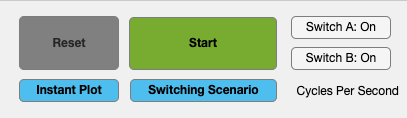
\includegraphics[width=10cm]{graphics/visualisation/ui_buttons}
     \caption{Buttons used in the visualisation interface}
\end{figure}

\paragraph{Switch Buttons}
\begin{itemize}
	\item The "Switch A" and "Switch B" buttons are used to turn on/off the primary and secondary switches in the multi-mode load respectively
	\item Pressing the button once will activate the switch.
	\item Once activated, pressing again will deactivate the switch.
	\item The combination of the switch states is used to determine the mode of operation.
\end{itemize}

\paragraph{Reset} The reset button is used to reset the simulation state. When it is pressed, the user is presented a dialog that the simulation has been reset. 
\begin{figure}[H]
     \centering
     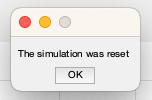
\includegraphics[width=5cm]{graphics/visualisation/dialog_reset}
     \caption{Dialog showing the user that the simulation has been reset}
\end{figure}
Resetting the simulation involves,
\begin{itemize}
	\item Clearing the graphs
	\item Resetting the RK4 initial values
	\item Resetting the time index
	\item Resetting the UI state
\end{itemize}

\paragraph{Start} The start button is used to start the simulation. When it is pressed, the program will begin to solve and plot the differential equations of the system, using RK4 over the specified duration and time step.
When the simulation is active,
\begin{itemize}
	\item The start button changes appearance to a pause button which can be used to stop, and later, resume the simulation
\begin{figure}[H]
     \centering
     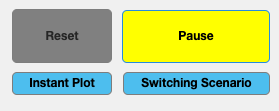
\includegraphics[width=10cm]{graphics/visualisation/pause_button}
     \caption{Dialog showing the user that the simulation has been reset}
\end{figure}
	\item The indicator is updated with a green light to show the simulation is running. The current mode of operation (determined by the switch buttons) is shown in the indicator.
\begin{figure}[H]
     \centering
     \begin{subfigure}[b]{0.45\textwidth}
         \centering
    	 
\includegraphics[width=2.5cm]{graphics/visualisation/ui_indicator_load}
     	\caption{Status indicator of the simulation while it is inactive under no load conditions}
     \end{subfigure}
     \hfill
     \begin{subfigure}[b]{0.45\textwidth}
         \centering
    	 
\includegraphics[width=3.5cm]{graphics/visualisation/ui_indicator_load_active}
     	\caption{Status indicator of the simulation while it is active under an inductive load}
     \end{subfigure}
     \hfill
\end{figure}
\end{itemize}

\paragraph{Instant Plot} Push button which instantly displays the plot at the final time chosen by the user. This plot will remain displayed until the user presses the reset button. 
\begin{figure}[H]
     \centering
     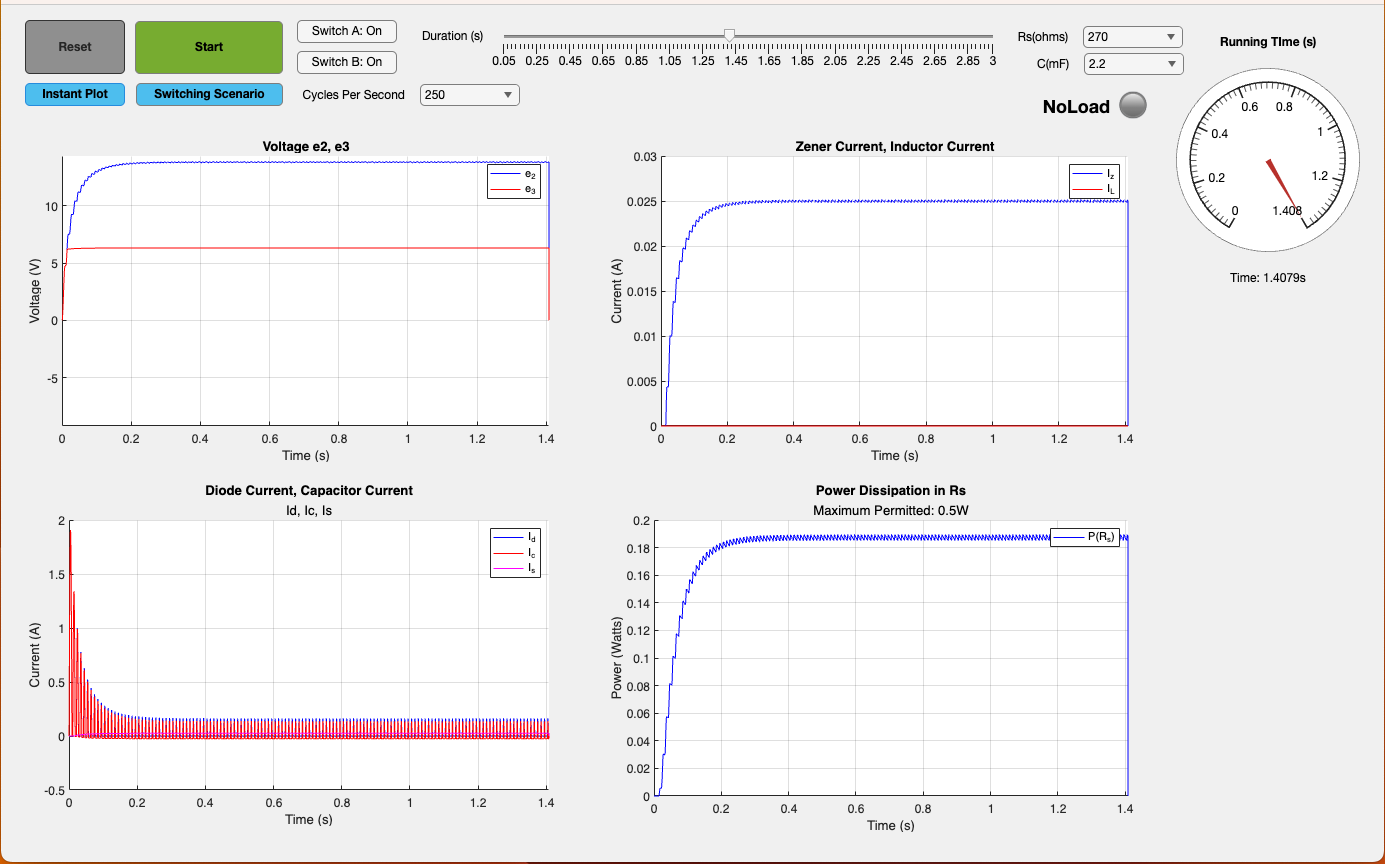
\includegraphics[width=\textwidth]{graphics/visualisation/no_load_instant_plot}
     \caption{The visualisation after pressing the Instant Plot button with no load conditions}
\end{figure}

\paragraph{Switching Scenario} Push button which when activated, triggers the switching scenario detailed in section \ref{section:switchingOperation}

\begin{figure}[H]
   \centering
   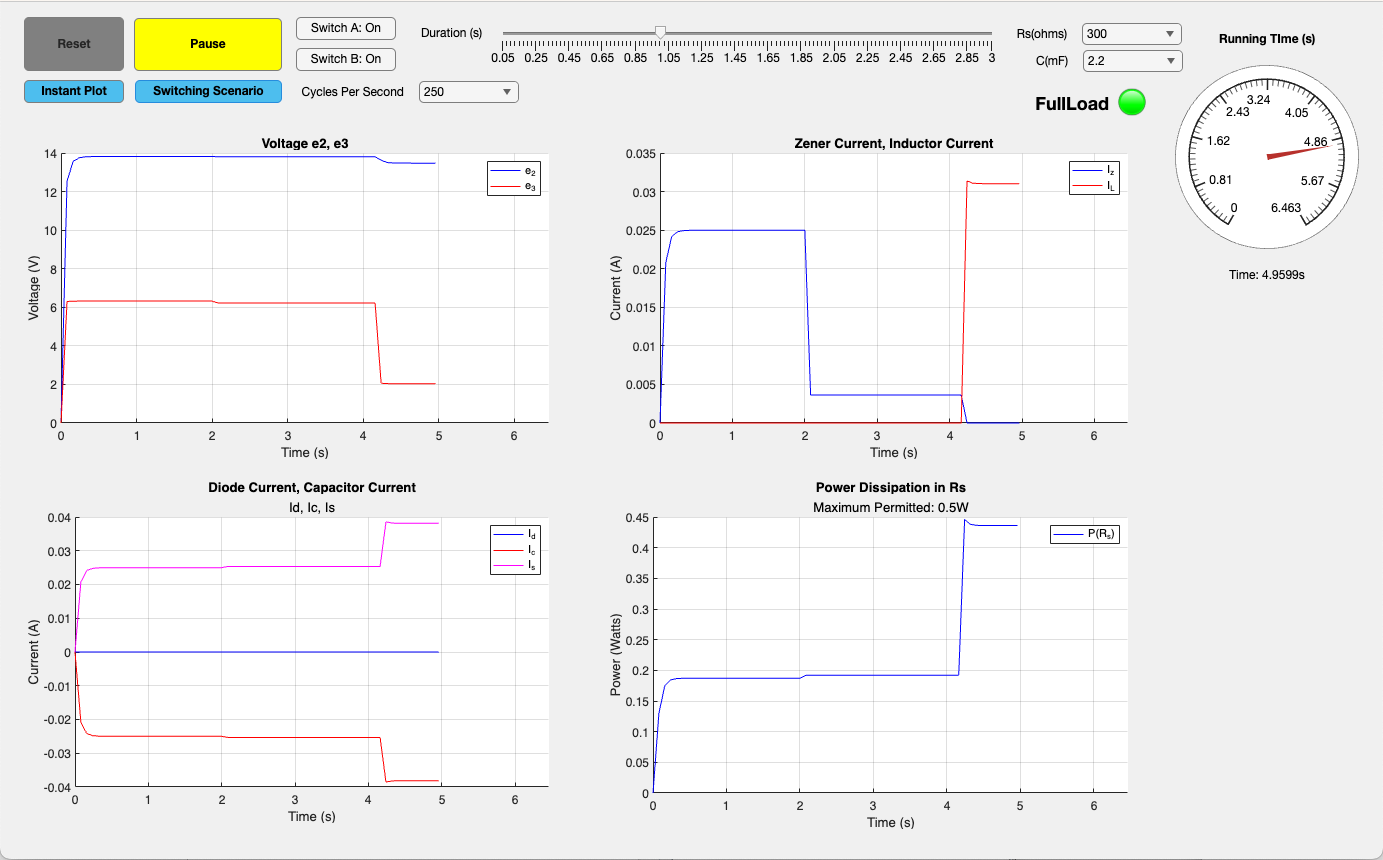
\includegraphics[width=0.95\textwidth]{graphics/visualisation/switching_3}
   \caption{The visualisation a few seconds after pressing the Switching Scenario button}
\end{figure}

\subsubsection{Dropdowns}
\begin{figure}[H]
     \centering
     \begin{subfigure}[b]{0.3\textwidth}
         \centering
    	 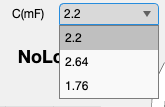
\includegraphics[width=\textwidth]{graphics/visualisation/ui_dropdowns_C}
     	\caption{Drop-down used to control the capacitance $C$ value}
     \end{subfigure}
     \hfill
     \begin{subfigure}[b]{0.3\textwidth}
         \centering
    	 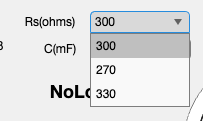
\includegraphics[width=\textwidth]{graphics/visualisation/ui_dropdowns_Rs}
     	\caption{Drop-down used to control the resistance $R_s$ value}
     \end{subfigure}
     \hfill
     \begin{subfigure}[b]{0.3\textwidth}
         \centering
    	 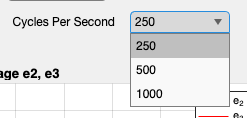
\includegraphics[width=\textwidth]{graphics/visualisation/ui_dropdowns_cycles}
     	\caption{Dropdown used to control the sampling rate $c$. Time step $h$ is determined using $\frac{T}{c}$}
     \end{subfigure}
     \hfill
\end{figure}
These values cannot be modified during the simulation. Doing so will result in the simulation being reset and the user must run the simulation again. A prompt will be shown if a change is detected while the simulation is active.
\begin{figure}[H]
     \centering
     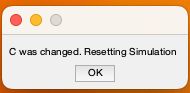
\includegraphics[width=5cm]{graphics/visualisation/dialog_cchange}
     \caption{Dialog showing the user that a change in $C$ was detected}
\end{figure}

\pagebreak
\subsubsection{Duration Slider} A slider which allows the user to change the duration of the simulation 

\begin{figure}[H]
    \centering
   	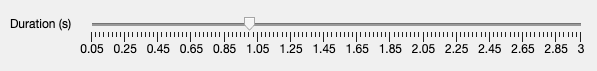
\includegraphics[width=\textwidth]{graphics/visualisation/ui_input_duration}
	\caption{Slider used to control the duration of the simulation}
\end{figure}

\subsubsection{Time Gauge} Working in tandem with the simulation, the time gauge monitors the elapsed time as the simulation advances. This enables the user to maintain a record of the time at specific plot points.

\begin{figure}[H]
    \centering
   	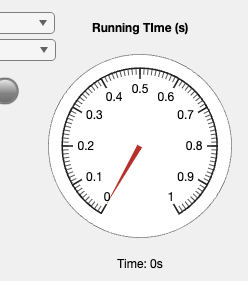
\includegraphics[width=5cm]{graphics/visualisation/ui_indicator_gage}
	\caption{Time gauge used to track the time progression of the simulation}
\end{figure}

\pagebreak
\subsection{Switching Operation} \label{section:switchingOperation}
The Switching Operation push button, integrated into the visualisation interface, serves the purpose of initiating a specific operation that fulfills the following condition
\begin{shquote}
The power supply is switched on at time $t=0$ at which the time the smoothing capacitor voltage and inductor current are zero, neither attached loading device is active at this time; after 2 sec the resistive load is switched on; after a further 2.2 sec the inductive load is switched in (i.e. connected) and it remains connected for the next 1.263 sec; subsequently the inductive device is switched out (i.e. disconnected) and remains disconnected
\end{shquote}

The visualisation was set up to support dynamic switching even while the simulation is running. When the user presses the Switch A and Switch B push buttons, the \texttt{comp.Mode} property is updated accordingly. This updated mode is then applied in the next iteration within the \texttt{updatePlot(comp)} function. Thus, the inductive and resistive loads can be connected and disconnected during the simulation, allowing for real-time changes. Implementing this scenario in the simulation was straightforward. It involved modifying the \texttt{comp.Mode} based on the current time value from the time index $k$.
\begin{table}[H]
    \centering
    \begin{tabular}{|c|c|}\hline
        Time (s) & \texttt{comp.Mode} \\\hline
        $t=0$ & NoLoad \\
        $2 < t < 4.2$ & ResistiveLoad \\
        $4.2 < t < 5.463$ & FullLoad \\
        $t > 5.463$ & ResistiveLoad \\\hline
    \end{tabular}
    \caption{How the \texttt{comp.Mode} value changes with respect to time for this switching operation}
    \label{tab:my_label}
\end{table}
\begin{lstlisting}[caption=Extract of code used to perform switching operation]
% Setup switching scenario
comp.SwitchingOperation = true;
            
% Power supply is switched off at t=0 neither attached loading
% device is active, Ic, IL=0
comp.ic = [0, 0, 0];
comp.Mode = CircuitMode.NoLoad;

% Use a larger time step to speed up
comp.TimeStep = 8e-5;

% Set time interval
t1 = 2; % tn + t1=time when mode=ResistiveLoad
t2 = 2.2; % tn + t2= time when mode=Full load
t3 = 1.263; % time in full load
tend = t1 + t2 + t3 + 1; % total time (add 1s for steady state at end)

% Time breaks
resistiveLoadTime = t1;
fullLoadTime = t1+t2;
revertTime = fullLoadTime+t3;

for n=comp.k:length(comp.t)-1
tn = comp.t(n)

% Check for current mode of operation based on time
if tn >= revertTime
  comp.mode = CircuitMode.ResistiveLoad;
elseif tn >= fullLoadTime
  comp.mode = CircuitMode.FullLoad;
elseif tn >= resistiveLoadTime
  comp.mode = CircuitMode.ResistiveLoad;
else
  comp.mode = CircuitMode.NoLoad;
end
	
% Update vin with time intervals
tn_1 = tn + comp.TimeStep;
tn_2 = tn + comp.TimeStep / 2;
vin = comp.v([tn, tn_1, tn_2]); 

% Perform RK4 simualtion
y = powerSupply(comp.mode,vin,h,comp.ic,comp.C,comp.Rs);  % Perform iteration
   
% Update initial conditions
comp.ic(1) = y.e2;
comp.ic(2) = y.e3;
comp.ic(3) = y.iL;
                
% Plot y-values ... 
end
\end{lstlisting}
\begin{figure}[H]
    \centering
   	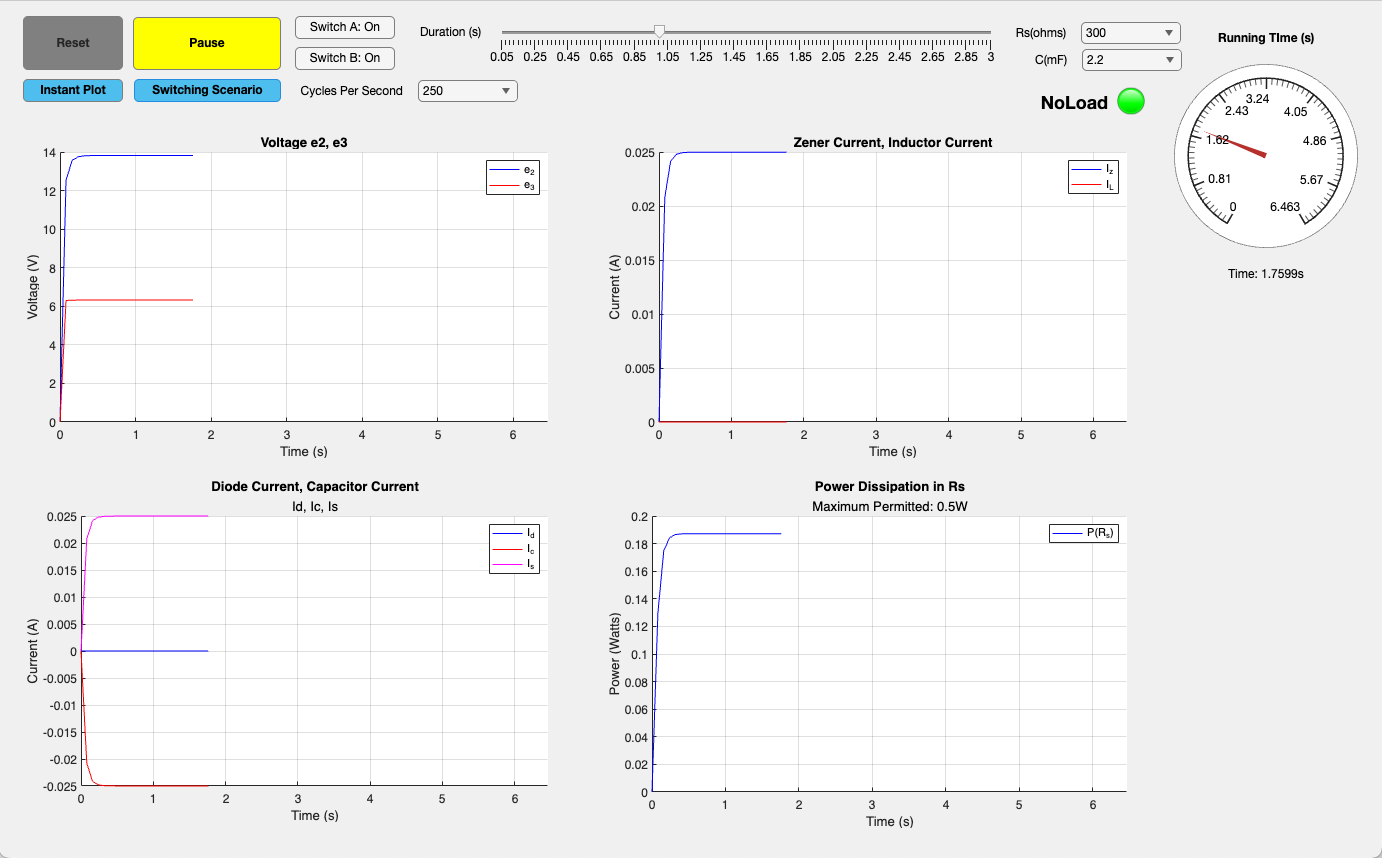
\includegraphics[width=\textwidth]{graphics/visualisation/switching_1}
	\caption{Visualisation at the beginning of the switching operation}
\end{figure}
\begin{figure}[H]
    \centering
   	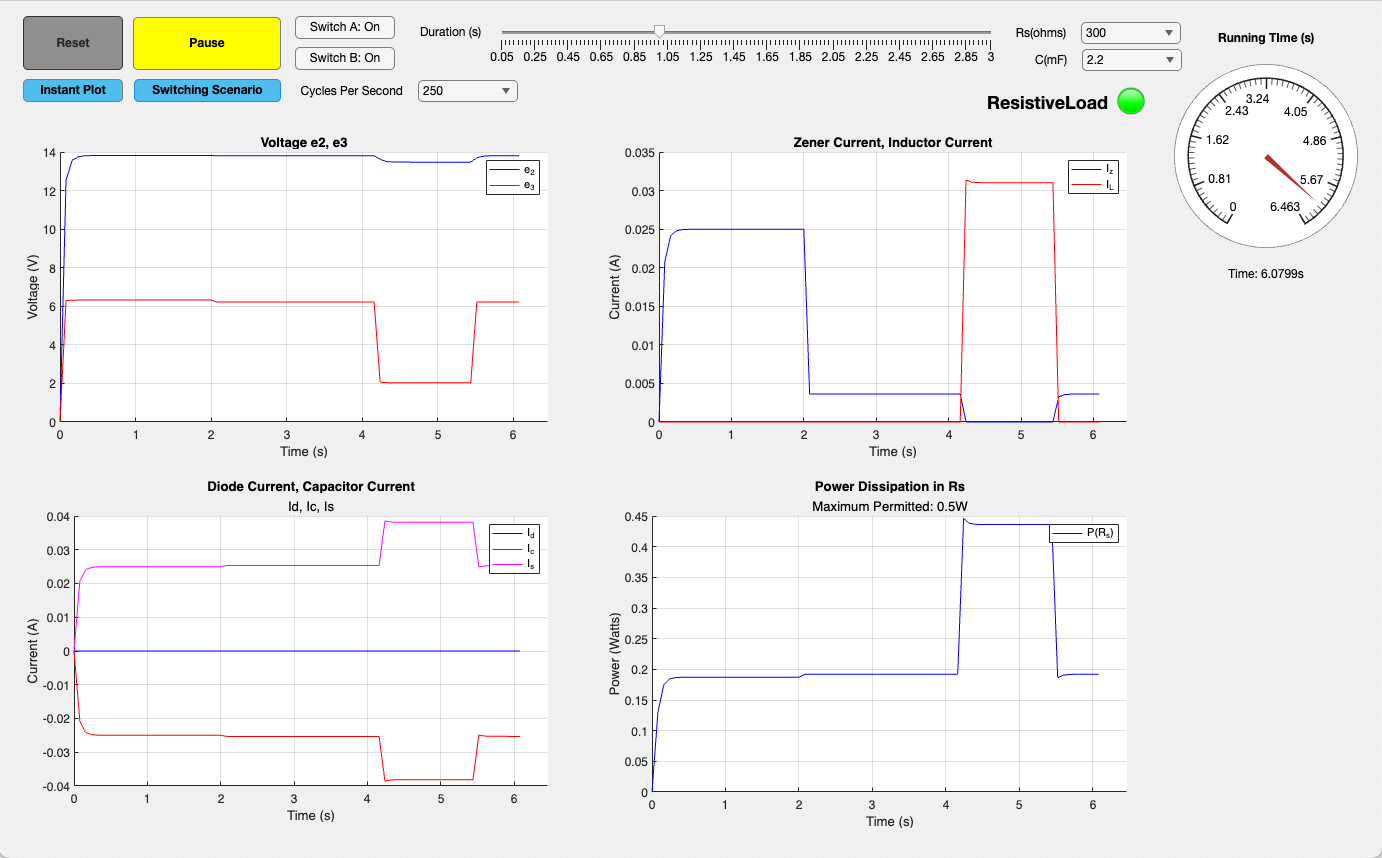
\includegraphics[width=\textwidth]{graphics/visualisation/switching_4}
	\caption{Visualisation towards the end of the switching operation}
\end{figure}
In general, the results of the switching operation align with predictions. After each incident, the circuit enters a transitory phase before stabilising into a consistent state following several cycles. The charge and discharge trajectories of the capacitor align with anticipated outcomes. The inductor's current becomes noticeable only when the inductive load is engaged, and it diminishes slightly upon reaching the stable state.


